\graphicspath{{results/fig/}}

\chapter{Implementation and results}
\label{chap:results}

    \section{Parameter estimation with practical data}
        \subsection{Mass estimation}
        \subsection{Simple payload cable length estimation}
        \subsection{Complex payload cable length estimation}

    \section{Data-driven system identification with practical data}

        \paragraph
        It was shown that the simulation environment 
        In Chapter~\ref{chap:system_id} it was shown that the data-driven methods 
        build accurate state prediction models for the considered system.
        It was also shown in Chapter~\ref{chap:modelling} that the simulation environment is a realistic representation of the practical system.
        However, there are still differences between simulations and practical flight.
        Therefore the data-driven algorithms are applied to practical flight data in this chapter 
        to investigate their performance in a practical implementation.

        \FloatBarrier\subsection{Methodology}

            \paragraph
            The methodology used to generate data with practical flights 
            follows the same general procedure as specified for simulation data in Section~\ref{sec:sys_id_methodology}:
            \begin{enumerate}
                \item Data logging starts when the quadrotor is armed
                \item Takeoff and hover with the qaudrotor
                \item Command velocity step setpoints
                \item Land the quadrotor
                \item Data logging stops when the quadrotor is disarmed
                \item Download data log from the quadrotor
                \item Split data into separate training and testing periods
                \item Build a model from the training data
                \item Calculate an error metric for the model from the testing data
            \end{enumerate}

            \begin{figure}[!htb]
                \centering
                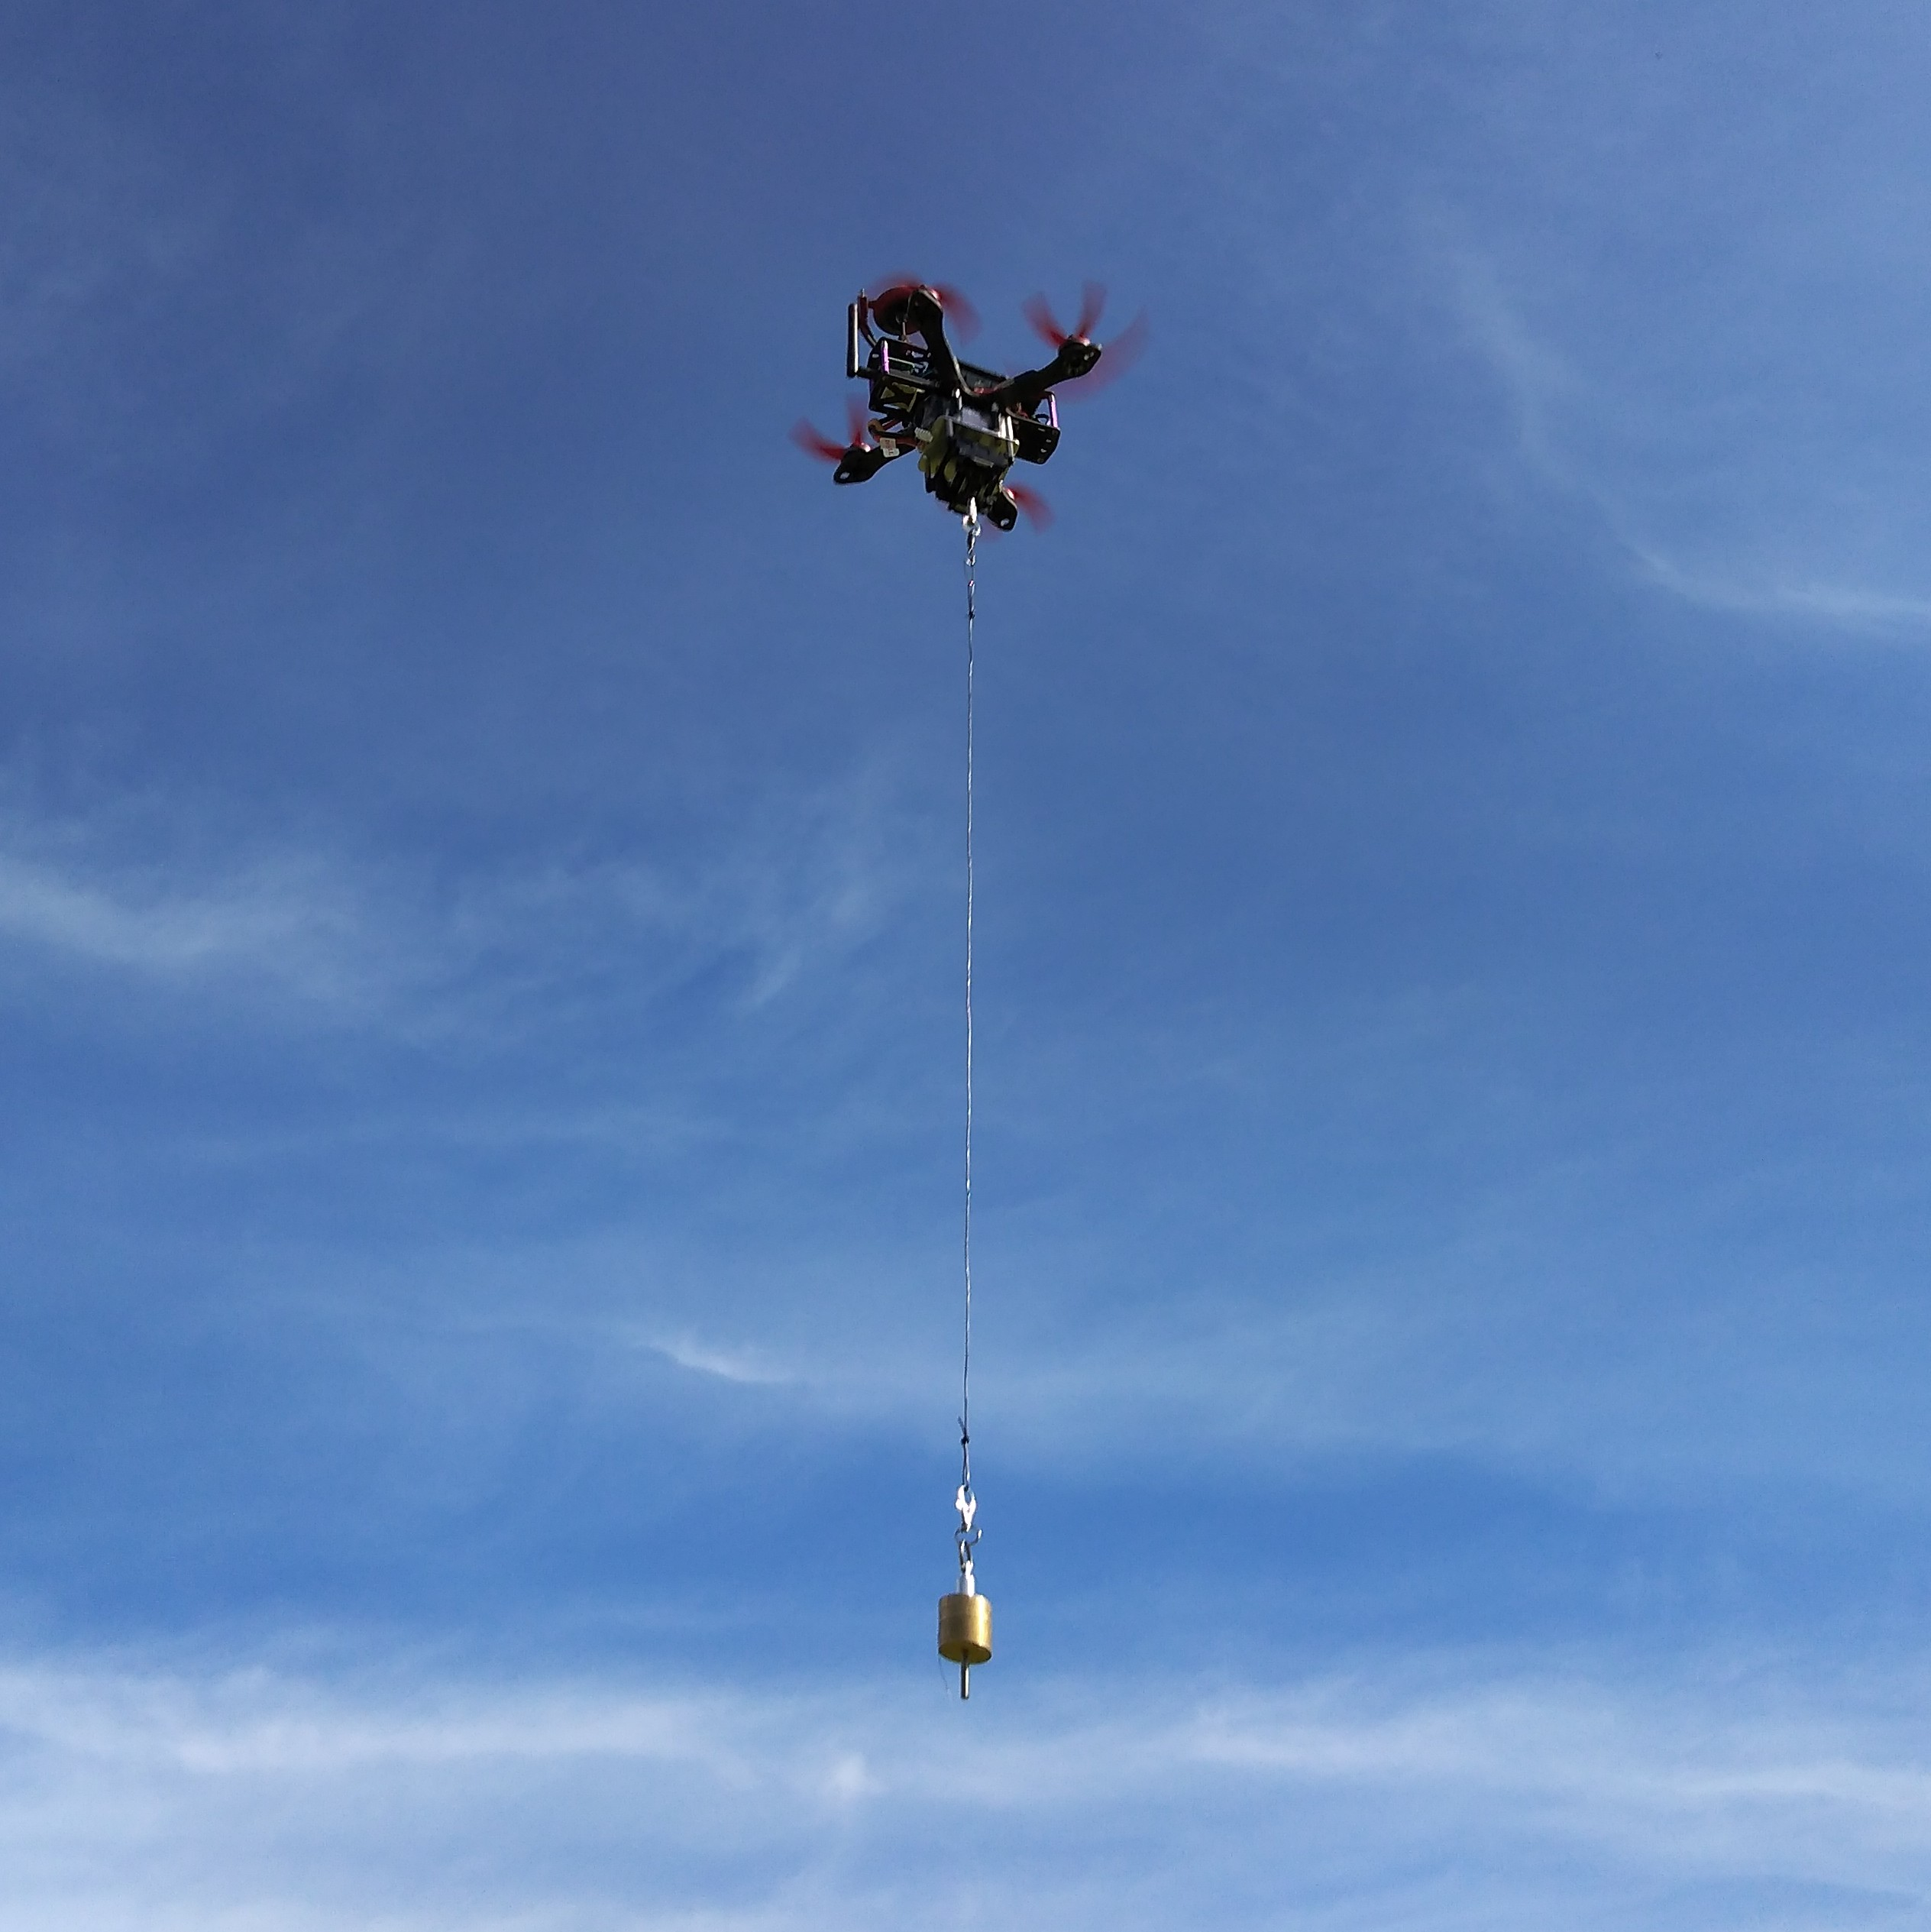
\includegraphics[width=0.5\linewidth]{honeybee_with_payload.jpg}
                \caption{Practical flight with Honeybee and a suspended payload}
                \label{fig:honeybee_with_payload}
            \end{figure}

            Figure~\ref{fig:honeybee_with_payload} shows Honeybee in flight with a suspended payload.
            Numerous flights were performed with different 
            payload masses, 
            cable lengths, 
            wind conditions, 
            and even with a more complex elongated payload.
            The system identification methods were then performed on the data resulting from this range of different use cases.
            The major differences between the simulations and practical flights involve the attachment of the payload and wind disturbances.
            In simulation, the payload cable is attached to the exact CoM of the quadrotor.
            However, due to practical constraints, the cable is attached slightly below the CoM of Honeybee.
            Practical flights are also influenced by wind disturbances, therefore this effect is also investigated in the sections below.
            In this chapter, wind conditions are referenced by the wind speed recorded by the website, www.yr.no, 
            for the hour of day of the flight.
            
            % \begin{itemize}
            %     \item Method for generating data
            %     \item Plot example of training data
            %     \item picture of practical flight single and double
            %     \item Discuss difference between SITL and prac
            %     \begin{itemize}
            %         \item Noise 
            %         \item wind
            %         \item CoM
            %     \end{itemize}
            %     \item plot hover of prac vs SITL to show noise and disturbance
            % \end{itemize}

            % \paragraph
            % In Chapter~\ref{chap:system_id} it was noted that the optimal length of training data 
            % often only included 2 velocity steps responses.
            % This means the models were trained on a very small sample of step sizes 
            % and need to extrapolate the dynamics of other step sizes.
        
            
        \FloatBarrier\subsection{Length of training data}

            \paragraph
            As discussed in Section~\ref{sec:sys_id_length_of_data}, 
            the length of training data used in the model has a large effect on prediction accuracy.
            The length of training data required for accurate models is largely influenced by the amount of wind disturbance during flight.
            Figure~\ref{fig:wind_Ttrain} shows prediction error as a function of training data length for different wind conditions.
            Its clear that the prediction error decreases with increasing wind speeds.
            It appears that for wind speeds lower than \SI{2}{\metre/\second}, 
            the minimum prediction error is not significantly improved with decreasing wind speeds.
            This may be because the flight dynamics is not significantly affected at such low wind speeds.
            
            \paragraph
            Wind adds an unmeasured input, also referred to as process noise, to the plant and this is not accounted for in the model.
            As discussed in Section~\ref{sec:noise}, the constant offset is subtracted from the acceleration setpoint data, 
            which results in a signal with a zero mean.
            This accounts for the constant component in the acceleration setpoint signal required to counteract the mean force of the wind.
            However, the wind speed deviates randomly from the mean speed which results in random process noise in the plant.

            % \paragraph
            % It appears that for higher wind speeds, 
            % the prediction error does not reach a peak value within the considered range of training data lengths.
            
            % This is expected, since the algorithms require longer lengths of training data to  
            
            \begin{figure}[htb]
    \centering
    \begin{tikzpicture}
        \begin{axis}[            
            xlabel = Length of training data,
            ylabel = $\overline{NMAE}$ \phantom{~},
            x unit = \si{\second},
            y unit = \%,
            xmin = 5,     xmax = 120,
            ymin = 3.2,  ymax = 15,
            grid = major,
            legend cell align = left,
            legend pos = north east,
            grid style = dashed,
            legend style = {font = \scriptsize},
            label style = {font = \scriptsize},
            tick label style = {font = \scriptsize},
            width = 0.95\columnwidth,
            height = 0.5\columnwidth,
            % initialize Dark2
            cycle list/Dark2,
            % combine it with 'mark list*':
            cycle multiindex* list = {
                Dark2\nextlist
            }
        ]

        \addplot+[mark = none, style = solid, ultra thick] 
        table[x = T_train, y expr = {\thisrow{NMAE_mean}*100}, col sep = comma] 
        {results/csv/NMAE_vs_Ntrain_Prac_2021-08-20_03_l-1_mp-0.2_wind-0.5.csv_dmd_angle.csv};
        \addlegendentry{0.5 m/s winds}

        \addplot+[mark = none, style = solid, ultra thick] 
        table[x = T_train, y expr = {\thisrow{NMAE_mean}*100}, col sep = comma] 
        {results/csv/NMAE_vs_Ntrain_Prac_2021-08-12_03_manual_x_vel_steps_2mps.csv_dmd_angle.csv};
        \addlegendentry{2 m/s winds}

        \addplot+[mark = none, style = solid, ultra thick] 
        table[x = T_train, y expr = {\thisrow{NMAE_mean}*100}, col sep = comma] 
        {results/csv/NMAE_vs_Ntrain_Prac_2021-08-12_02_manual_x_vel_steps_4mps.csv_dmd_angle.csv};
        \addlegendentry{4 m/s winds}

        \addplot+[mark = none, style = solid, ultra thick] 
        table[x = T_train, y expr = {\thisrow{NMAE_mean}*100}, col sep = comma] 
        {results/csv/NMAE_vs_Ntrain_Prac_2021-08-26_01_l-1_mp-0.2_wind-6.csv_dmd_angle.csv};
        \addlegendentry{6 m/s winds}

        \end{axis}
    \end{tikzpicture} 
    
    \caption{Effect of wind on \gls{DMD} prediction errors for different lengths of practical training data
    ($m_p =$~\SI{0.2}{\kilo\gram}, $l =$~\SI{1}{\meter}, $T_s =$~\SI{0.03}{\second}).}
    \label{fig:wind_Ttrain}
\end{figure}

            
            \paragraph
            HAVOK and DMD perform similarly
            Figure~\ref{fig:havok_vs_dmd_Ttrain_2mps} shows the prediction error of DMD and HAVOK models
            
            \begin{figure}[htb]
    \centering
    \begin{tikzpicture}
        \begin{axis}[            
            xlabel = Length of training data,
            ylabel = $\overline{NMAE}$ \phantom{~},
            x unit = \si{\second},
            y unit = \%,
            xmin = 5,     xmax = 120,
            ymin = 3.2,  ymax = 15,
            grid = major,
            legend cell align = left,
            legend pos = north east,
            grid style = dashed,
            legend style = {font = \scriptsize},
            label style = {font = \scriptsize},
            tick label style = {font = \scriptsize},
            width = 0.95\columnwidth,
            height = 0.5\columnwidth,
            % initialize Dark2
            cycle list/Dark2,
            % combine it with 'mark list*':
            cycle multiindex* list = {
                Dark2\nextlist
            }
        ]

        \addplot+[mark = none, style = solid, ultra thick] 
        table[x = T_train, y expr = {\thisrow{NMAE_mean}*100}, col sep = comma] 
        {results/csv/NMAE_vs_Ntrain_Prac_2021-08-12_03_manual_x_vel_steps_2mps.csv_dmd_angle.csv};
        \addlegendentry{DMD}

        \addplot+[mark = none, style = solid, ultra thick] 
        table[x = T_train, y expr = {\thisrow{NMAE_mean}*100}, col sep = comma] 
        {results/csv/NMAE_vs_Ntrain_Prac_2021-08-12_03_manual_x_vel_steps_2mps.csv_havok_angle.csv};
        \addlegendentry{HAVOK}

        \end{axis}
    \end{tikzpicture} 
    
    \caption{\gls{DMD} and \gls{HAVOK} prediction errors for different lengths of practical training data
    ($m =$~\SI{0.206}{\kilo\gram}, $l =$~\SI{1}{\meter}, $T_s =$~\SI{0.03}{\second}).}
    \label{fig:havok_vs_dmd_Ttrain_2mps}
\end{figure}


            Also plot DMD vs HAVOK for high winds ??
            

            plot NMAE vs Ttrain
            \begin{itemize}
                \item Plot strong wind vs less wind vs no wind
                \item HAVOK vs DMD
                \item Plot single pend vs double pend
            \end{itemize}
            
        \FloatBarrier\subsection{Hyperparameters}
            
            \paragraph
            As discussed in Section~\ref{sec:sec:hyperparameters}, 
            the prediction error improves with an increasing number of delay-coordinates, but reaches 

            \begin{figure}[htb]
    \centering
    \begin{tikzpicture}
        \begin{axis}[            
            xlabel = {Number of delay-coordinates, $q$},
            ylabel = $\overline{NMAE}$ \phantom{~},
            % x unit = \si{\second},
            y unit = \%,
            xmin = 5,     xmax = 90,
            ymin = 3.5,  ymax = 7.5,
            grid = major,
            legend cell align = left,
            legend pos = north east,
            grid style = dashed,
            legend style = {font = \scriptsize},
            label style = {font = \scriptsize},
            tick label style = {font = \scriptsize},
            width = 0.95\columnwidth,
            height = 0.5\columnwidth,
            % initialize Dark2
            cycle list/Dark2,
            % combine it with 'mark list*':
            cycle multiindex* list = {
                Dark2\nextlist
            }
        ]

        \addplot+[mark = none, style = solid, ultra thick] 
        table[x = q, y expr = {\thisrow{NMAE_mean}*100}, col sep = comma] 
        {results/csv/NMAE_vs_q_Prac_2021-08-12_03_manual_x_vel_steps_2mps_q.csv_dmd_angle.csv};
        \addlegendentry{DMD}

        \addplot+[mark = none, style = solid, ultra thick] 
        table[x = q, y expr = {\thisrow{NMAE_mean}*100}, col sep = comma] 
        {results/csv/NMAE_vs_q_Prac_2021-08-12_03_manual_x_vel_steps_2mps_q.csv_havok_angle.csv};
        \addlegendentry{HAVOK}

        % \addplot+[mark = none, style = solid, ultra thick] 
        % table[x = q, y expr = {\thisrow{NMAE_mean}*100}, col sep = comma] 
        % {results/csv/NMAE_vs_q_Prac_2021-08-20_03_l-1_mp-0.2_wind-0.5_q.csv_dmd_angle.csv};
        % \addlegendentry{DMD}

        % \addplot+[mark = none, style = solid, ultra thick] 
        % table[x = q, y expr = {\thisrow{NMAE_mean}*100}, col sep = comma] 
        % {results/csv/NMAE_vs_q_Prac_2021-08-20_03_l-1_mp-0.2_wind-0.5_q.csv_havok_angle.csv};
        % \addlegendentry{HAVOK}


        \end{axis}
    \end{tikzpicture} 
    
    \caption{\gls{DMD} and \gls{HAVOK} prediction errors for different number of delays included in the model
    ($m =$~\SI{0.206}{\kilo\gram}, $l =$~\SI{1}{\meter}, $T_s =$~\SI{0.03}{\second}, wind speed $\approx~$\SI{2}{\metre/\second}).}
    \label{fig:havok_vs_dmd_q_2mps}
\end{figure}


            \begin{figure}[htb]
    \centering
    \begin{tikzpicture}
        \begin{semilogyaxis}[            
            xlabel = Index of mode,
            ylabel = Singular value,
            % x unit = \si{\second},
            % y unit = \si{\second},
            xmin = 0,     xmax = 183,
            ymin = 1e-5,  ymax = 1e4,
            grid = major,
            legend cell align = left,
            legend pos = north east,
            grid style = dashed,
            legend style = {font = \scriptsize},
            label style = {font = \scriptsize},
            tick label style = {font = \scriptsize},
            width = 0.95\columnwidth,
            height = 0.5\columnwidth,
            % initialize Dark2
            cycle list/Dark2,
            % combine it with 'mark list*':
            cycle multiindex* list = {
                Dark2\nextlist
            }
        ]

        \addplot+[only marks, mark = *, ultra thin, mark options={scale=0.7}] 
        table[x = index, y = S, col sep = comma] 
        {results/csv/Singular_values_Prac_2021-08-12_03_manual_x_vel_steps_2mps_q.csv_havok_angle_Ttrain_50_q91_p52.csv};
        \addlegendentry{Significant modes}

        \addplot+[only marks, mark = *, ultra thin, mark options={scale=0.7}] 
        table[x = index, y = S, col sep = comma] 
        {results/csv/Singular_values_Prac_2021-08-12_03_manual_x_vel_steps_2mps_q.csv_havok_angle_Ttrain_50_q91_p52_trunc.csv};
        \addlegendentry{Truncated modes}

        \end{semilogyaxis}
    \end{tikzpicture} 
    
    \caption{Significant and truncated singular values of a \gls{HAVOK} model produced from practical data
    ($m_p =$~\SI{0.2}{\kilo\gram}, $l =$~\SI{0.5}{\meter}, $T_s =$~\SI{0.03}{\second}, $T_{train} =$~\SI{60}{\second}.)}
    \label{fig:prac_singular_values}
\end{figure}


            Difference between SITl and practical (same input steps)
            This is due to wind disturbance
            Plot wind vs less wind vs no wind
            
        \FloatBarrier\subsection{System parameters}

            \paragraph
            It was shown with multiple simulations in Section~\ref{sec:system_params} 
            that the system identification methods work for a range of different payload parameters.
            Figure~\ref{fig:prac_system_params} shows the prediction error for different payloads with practical data.
            This shows that the proposed methods also work in practice with different payloads.
            
            % \begin{figure}[htb]
    \centering
    \begin{tikzpicture}
        \begin{axis}[            
            xlabel = Length of training data,
            ylabel = $\overline{NMAE}$ \phantom{~},
            x unit = \si{\second},
            y unit = \%,
            xmin = 5,     xmax = 120,
            ymin = 2.8,  ymax = 7.8,
            grid = major,
            legend cell align = left,
            legend pos = north east,
            grid style = dashed,
            legend style = {font = \scriptsize},
            label style = {font = \scriptsize},
            tick label style = {font = \scriptsize},
            width = 0.95\columnwidth,
            height = 0.5\columnwidth,
            % initialize Dark2
            cycle list/Dark2,
            % combine it with 'mark list*':
            cycle multiindex* list = {
                Dark2\nextlist
            }
        ]
         
        \addplot+[mark = none, style = solid, ultra thick] 
        table[x = T_train, y expr = {\thisrow{NMAE_mean}*100}, col sep = comma] 
        {results/csv/NMAE_vs_Ntrain_Prac_2021-08-20_01_l-1_mp-0.1_wind-0.5.csv_dmd_angle.csv};
        \addlegendentry{$m =$~\SI{0.1}{\kilo\gram}, $l = $~\SI{1}{\metre}}
        
        \addplot+[mark = none, style = solid, ultra thick] 
        table[x = T_train, y expr = {\thisrow{NMAE_mean}*100}, col sep = comma] 
        {results/csv/NMAE_vs_Ntrain_Prac_2021-08-20_02_l-2_mp-0.3-wind-0.5.csv_dmd_angle.csv};
        \addlegendentry{$m =$~\SI{0.3}{\kilo\gram}, $l = $~\SI{2}{\metre}}
        
        \addplot+[mark = none, style = solid, ultra thick] 
        table[x = T_train, y expr = {\thisrow{NMAE_mean}*100}, col sep = comma] 
        {results/csv/NMAE_vs_Ntrain_Prac_2021-08-20_03_l-1_mp-0.2_wind-0.5.csv_dmd_angle.csv};
        \addlegendentry{$m =$~\SI{0.2}{\kilo\gram}, $l = $~\SI{1}{\metre}}
        
        \end{axis}
    \end{tikzpicture} 

    \caption{DMD prediction error as a function of training data length for different payload parameters}
    \label{fig:prac_system_params}
\end{figure}


            \paragraph
            Plot NMAE vs Ttrain - 1 graph
            \begin{itemize}
                \item m = 0.2 kg    l = 1 m  
                \item m = 0.2 kg    l = 2 m
                \item l = 1 m       m = 0.3 kg
                \item l = 1 m       m = 0.1 kg
            \end{itemize}

        \FloatBarrier\subsection{Predictions}
            \begin{itemize}
                \item Single pendulum: Plot 4 in grid showing good and bad
                \item Double pendulum: Plot 4 in grid showing good and bad
            \end{itemize}

            Predictions drift because of the changing acceleration setpoint vector required.
            plot hover of prac vs SITL to show noise and disturbance

        % \FloatBarrier\subsection{Extended dimensions}
        %     \begin{itemize}
        %         \item plot error vs T-train for XY
        %         \item plot predictions
        %         \item plot error vs T-train for XYZ
        %     \end{itemize}
        % Maybe add this is there is time??
            
    \section{Swing damping control systems}

        \paragraph
        After the system identification phase, active swing damping control can be applied
        to the quadrotor and payload system.
        The control architectures are summarised in Table~\ref{tbl:controller_summary} 
        by pairing the system identification techniques along with the appropriate controllers.
        It was firstly shown in Chapter~\ref{chap:system_id} that the system identifcation techniques worked in simulation.
        Emphasise that control is now applied in full SITL simulation.

        \paragraph
        MATLAB is used to generate a MPC ROS node 
        This ROS node receives state feedback from the Gazebo simulator,
        computes the optimal control action,
        and send the setpoint to PX4 through the package 'mavros'.

        \begin{table}[!h]
            \renewcommand{\arraystretch}{1.1}
            \centering
            \caption{Summary of the system identification techniques paired with the active damping controllers.}
            \begin{tabularx}{0.75\linewidth}{@{}lll@{}}
                \toprule
                \multicolumn{2}{c}{\textbf{System identification}}   & \textbf{Controller} \\
                \cmidrule(lr){1-2}
                Category    & Algorithm                     & \\
                \midrule
                White-box   & RLS mass estimator, and       & LQR \\
                            & FFT cable length estimator    & \\
                Black-box   & DMDc, or                      & MPC \\
                            & HAVOK                         & \\
                \bottomrule
            \end{tabularx}
            \label{tbl:controller_summary}
        \end{table}
        

        \FloatBarrier\subsection{Single pendulum}

            \begin{itemize}
                \item subplot prediction of data driven model. subplot prediction of white-box model
                \item plot MPC vs LQR v PID (no wind) step = 1 m/s
                \item plot MPC vs LQR v PID (no wind) step = 2 m/s
                \item plot DMDc vs HAVOK (DMD - Havok)
                \item plot with wind disturbacne control
            \end{itemize}

        \FloatBarrier\subsection{Double pendulum}

            \begin{itemize}
                \item subplot prediction of data driven model. subplot prediction of white-box model
                \item plot MPC vs LQR v PID (no wind)
                \item plot DMDc vs HAVOK (DMD - Havok)
            \end{itemize}

    \section{HIL}

    \section{Conclusion}


